%version corregida de analisis

\chapter{Análisis}

En esta sección, analizamos los datos obtenidos para entrenar clasificadores que distingan entre hablantes de Buenos Aires y Córdoba. Recordemos que tomamos las 260 grabaciones obtenidas a través de la página web y les aplicamos el extractor de atributos descripto en el capítulo 4. El resultado nos dio la descripción de cada grabación a través de los atributos que definimos. 

Primero presentaremos el baseline que consideramos. Este nos servirá para tener una clasificación aceptable que luego trataremos de superar. Explicaremos los clasificadores utilizados para vencer esta marca y en base a tests estadísticos notaremos si aportan datos significativos. También describiremos el modelo de testing utilizando los datos recolectados. Por último, analizamos los atributos más descriptivos del habla de Buenos Aires y Córdoba. 

Para el análisis de los datos, utilizamos la herramienta Weka\footnote{Página web: http://www.cs.waikato.ac.nz/ml/weka/}. Ésta provee varios algoritmos de machine learning. Para los tests estadísticos utilizamos la herramienta R versión 3.0.1. 

\section{Baseline}

El baseline define el clasificador más simple, que posteriormente tratamos de vencer. No encontramos ningún trabajo que trate de distinguir entre porteños y cordobeses a partir de su habla. Es por eso que definimos el baseline utilizando el algoritmo \textbf{majority class}. Este algoritmo clasifica eligiendo siempre la categoría que en el conjunto es mayoritaria. Por ejemplo, si nuestro conjunto de datos de train tiene más muestras de Córdoba para la clasificación de nuevas instancias elegimos siempre Córdoba. La herramienta Weka provee un clasificador basado en majority class llamado \textbf{ZeroR}. Utilizaremos este para el cálculo del baseline. 

Recordemos que, como vimos en el capítulo anterior, el conjunto de datos que obtuvimos posee más grabaciones de Buenos Aires que de Córdoba. Utilizando nuestros datos, este baseline tuvo una performance alrededor del 69\% de efectividad. Nos referimos a efectividad como la probabilidad de clasificar correctamente un hablante. Éste fue el porcentaje a superar. Si nuestro conjunto de datos estuviera debidamente balanceado este porcentaje sería exactamente del 50\% ya que, al elegir la clase mayoritaria, ninguna de las clases superaría a la otra. Lo ideal sería poder tener misma cantidad de los dos grupos. Al tener este desbalance, puede suceder que al clasificar a un hablante en un test se obtengan mejores resultados para Buenos Aires que para Córdoba, ya que tengo más muestras para identificar a un hablante. Esto se verá en detalle más adelante.

\section{Clasificadores}

Entrenamos varios clasificadores para poder determinar la procedencia de un hablante y superar la performance del clasificador baseline. Elegimos varios clasificadores de distintos tipos para éste propósito. 

Recordemos que para cada grabación sólo se determinan los atributos que esa frase define y los demás quedan en valor desconocido. Es por ello, que nuestros clasificadores van a tener que manejar atributos desconocidos. Algunos clasificadores tienen la posibilidad de trabajar con estos atributos de forma natural, otros no. 

Describimos cómo trabaja cada clasificador y además cómo trabaja con los valores desconocidos. Los clasificadores propuestos son: 

\subsubsection*{Repeated Incremental Pruning to Produce Error Reduction (RIPPER) \cite{Cohen1995} - Implementación JRip:}

%http://weka.sourceforge.net/doc.dev/weka/classifiers/rules/JRip.html
%http://www.cs.utsa.edu/~bylander/cs6243/cohen95ripper.pdf
%https://indico.cern.ch/event/34666/session/13/material/slides/0?contribId=16 pag 21

Este algoritmo intenta describir el conjunto de entrada definiendo pequeños grupos. Primero localiza un grupo que posee la característica a clasificar, y genera reglas que lo describan. Va agregando reglas de forma golosa. Luego cuando se supera una cierta condición (por ejemplo: cantidad de reglas), lo extrae y sigue con otro grupo. Finaliza cuando describe todos los grupos del conjunto de entrada. Entonces la forma de clasificar es definiendo una serie de reglas lógicas utilizando los atributos.

Cuando se producen las reglas en la fase de entrenamiento, las instancias que poseen atributo indefinido para la regla que se esta armando no son consideradas para el armado de la misma, o sea no se toman en consideración para las variables internas del algoritmo. Esto tiene la ventaja de que se dejan de lado para el final: primero se arman las reglas para las instancias que sí pueden ser clasificadas y luego, quedan solamente las instancias con valores indefinidos, pudiendo ser más fácil el armado de una regla que las identifique.  

Si al momento de clasificar, una instancia posee un atributo desconocido y éste es necesario para una determinada regla de decisión, esta regla falla y sigue con la siguiente regla. Se evalúa la próxima regla de la misma forma hasta llegar a una posible clasificación.

\subsubsection*{C4.5 \cite{Quinlan1993} - Implementación J48:}

%http://en.wikipedia.org/wiki/C4.5_algorithm
%http://weka.sourceforge.net/doc.dev/weka/classifiers/trees/J48.html

Este algoritmo se basa en un árbol de decisión. Tenemos nuestro conjunto de entrenamiento con instancias clasificadas y cada una de estas instancias consiste en un vector con sus atributos. El algoritmo realiza lo siguiente: para cada nodo del árbol se elige el atributo que efectivamente mejor separa a los dos grupos. El criterio para encontrar este atributo es utilizando la ganancia de información de cada atributo. El atributo con la mayor ganancia de información es utilizado como nodo del árbol. Luego se llama recursivamente por cada subconjunto que dividimos. Si las muestras pertenecen a la misma clase o los atributos no proveen información se crea sólo una hoja.

Las instancias que poseen valores indefinidos para el atributo que mejor separa en subgrupos no son separados ni en uno ni en otro subconjunto, sino que son utilizados en ambos. Entonces estas instancias en este paso no aportan diferencia entre una rama u otra. Lo interesante es que más adelante, calculando otro nodo del árbol, sí pueden ir a un subconjunto específico.

Si al momento de clasificar una instancia, el árbol utiliza un atributo desconocido se realiza lo siguiente: propaga por cada rama del nodo hacia abajo pero en cada camino sigue con un peso proporcional a la cantidad de elementos que fueron por cada rama en el entrenamiento. Luego, al llegar a los nodos hoja, combina los resultados utilizando esos pesos y elige la clase con mayor peso.

\subsubsection*{Support Vector Machine \cite{Platt98sequentialminimal} - Implementación Function SMO:}

%http://en.wikipedia.org/wiki/Support_vector_machine
%http://machinelearning.wustl.edu/mlpapers/paper_files/BordesEWB05.pdf
%http://en.wikipedia.org/wiki/Sequential_minimal_optimization
%http://research.microsoft.com/pubs/69644/tr-98-14.pdf

Support vector machine define uno o varios hiperplanos para intentar clasificar muestras. Este hiperplano se construye utilizando transformaciones lineales de los datos de entrada y sirve para clasificar las muestras en dos grupos. Utilizando este hiperplano, se puede etiquetar cada dato de entrada con su clasificación observando de qué lado del hiperplano se encuentra.

Este algoritmo no puede ejecutarse si se posee instancias con atributos desconocidos. Es por eso que antes de empezar el entrenamiento a cada instancia con atributos que poseen valores desconocidos se la define con el valor de la media de ese atributo de las demás instancias. De esta forma, vamos a otorgarle un lugar aproximado en el hiperplano para ese atributo. Esto también sucede si al momento de clasificar la instancia posee un atributo desconocido.  

\subsubsection*{Naive Bayes \cite{DBLP:conf/flairs/Zhang04} - Implementación homónima:}

%http://www.cs.unb.ca/profs/hzhang/publications/FLAIRS04ZhangH.pdf
%http://en.wikipedia.org/wiki/Naive_Bayes_classifier

Un clasificador de tipo Naive Bayes supone que cada atributo describe una característica de su clase y no está relacionado con otro atributo. Cada uno de estos atributos contribuye de manera independiente a la clasificación de su clase. Se define una regla de decisión utilizando un modelo probabilístico basado en el teorema de Bayes para la clasificación de cada grupo.

Si un valor es indefinido en una instancia de entrenamiento, simplemente no es incluida para el cálculo de la clasificación. Los valores que son tenidos en cuenta son los que están definidos, o sea los que ocurren realmente. Esto es posible gracias a que los atributos son tenidos en cuenta como independientes.

\section{Tests estadísticos}

Utilizamos los resultados de cada clasificador para ver si son significativamente relevantes en la predicción de cada hablante en comparación con el baseline. Para realizar estos tests utilizamos para cada clasificador un vector con los porcentajes de instancias correctas para cada fold generado\footnote{Veremos cómo se componen los distintos folds más adelante en la sección \ref{modelos_tests}}. Los clasificadores utilizados son los descriptos en la sección anterior más el baseline. Para estos resultados realizamos dos tests principales: Prueba de rangos con signo de Wilcoxon y Test t de Student. 

\subsection{Test de Wilcoxon}

Utilizamos el test de Wilcoxon ya que no estamos seguros que nuestros datos provengan de una distribución Normal. Este nos ayudará a determinar si hay razones estadísticas para decir si un clasificador es distinto que otro. Para realizar este test armamos un vector para cada clasificador incluyendo el baseline. Este vector tendrá el porcentaje de instancias correctas para cada uno de los folds. Entonces correremos el test estadístico utilizando el vector del clasificador baseline y el vector de otro clasificador, por ejemplo Support vector machine.

%TODO: comentar que esto lo saqué
%Para realizar este test se debe cumplir que:
%
%\begin{itemize}
%	%Data are paired and come from the same population.
%	\item Los datos son presentados de a pares y vienen de la misma población: esto sucede gracias a cómo generamos los tests. La población también siempre es la misma.
%	%Each pair is chosen randomly and independently.
%	\item Cada par es elegido al azar e independiente del resto: cada grupo generado para testing está armado de forma azarosa ya que la elección de cada hablante se realiza de esta forma. 
%	%TODO: Tratamos de maximizar la independencia entre folds.
%	%ojo acá hay que tener mucho cuidado con el primer test estadistico el de la primer versión
%	
%	%The data are measured at least on an ordinal scale, but need not be normal.
%	\item Los datos están medidos sobre una escala ordinal y no necesariamente debe provenir de una distribución Normal: esta característica es fundamental ya que, como dijimos, no estamos seguros que nuestros datos provengan de una distribución Normal.
%\end{itemize}

Las hipótesis fueron:

\vspace{0.5cm}
\hspace{2cm}$H_0$: Clasificador alternativo no es diferente que ZeroR
\vspace{0.25cm}

\hspace{2cm}$H_1$: Clasificador alternativo es diferente que ZeroR
\vspace{0.5cm}

Clasificador alternativo se refiere a los demás clasificadores descriptos. 

Cada uno de los tests nos va a dar un p-valor. Si este es mayor 0,05, consideramos que no hay evidencia suficiente para determinar que el clasificador alternativo es mejor. Si de lo contrario es menor, sí podemos rechazar $H_0$ y asegurar que el alternativo es mejor. 

%Luego chequeamos si nuestra muestra corresponde a una distribución Normal. Para chequear Normalidad utilizamos el test de Shapiro-Wilk.

\subsection{Análisis Shapiro-Wilk Test}

%todo: pensar si debo explicar todo el metodo o no hace falta
%http://es.wikipedia.org/wiki/Test_de_Shapiro%E2%80%93Wilk

%En estadística, el Test de Shapiro–Wilk se usa para contrastar la normalidad de un conjunto de datos. Se plantea como hipótesis nula que una muestra x1, ..., xn proviene de una población normalmente distribuida. Fue publicado en 1965 por Samuel Shapiro y Martin Wilk.1 Se considera uno de los test más potentes para el contraste de normalidad, sobre todo para muestras pequeñas (n<30).

Utilizamos el test de Shapiro-Wilk para poder afirmar si un conjunto de datos proviene de una distribución Normal.

%Interpretación: Siendo la hipótesis nula que la población está distribuida normalmente, si el p-valor es menor a alfa (nivel de confianza) entonces la hipótesis nula es rechazada (se concluye que los datos no vienen de una distribución normal). Si el p-valor es mayor a alfa, no se rechaza la hipótesis y se concluye que los datos siguen una distribución normal.

El test de Shapiro-Wilk se basa en plantear como hipótesis nula que la población está distribuida de forma Normal. Aplicamos el estadístico de este test: si el p-valor nos da menor a 0,05 entonces la hipótesis nula es rechazada y se afirma que los datos no provienen de una distribución Normal. Si, en cambio, es mayor a 0,05 no hay evidencia suficiente para rechazar $H_0$ y por ende se afirma que los datos siguen una distribución Normal.

Este test se realiza individualmente para cada vector resultado de porcentaje de instancias correctas para cada clasificador. O sea, chequeamos que los resultados de cada clasificador se asemejen a la distribución Normal. Por ejemplo si los resultados de ambos clasificadores ZeroR y J48 tuvieron en el test Shapiro-Wilk un p-valor mayor a 0,05, se puede realizar el t de Student para ellos dos. En caso contrario, se debe usar el test de Wilcoxon.

\subsection{Student t Test}

%En estadística, una prueba t de Student, prueba t-Student, o Test-T es cualquier prueba en la que el estadístico utilizado tiene una distribución t de Student si la hipótesis nula es cierta. Se aplica cuando la población estudiada sigue una distribución normal pero el tamaño muestral es demasiado pequeño como para que el estadístico en el que está basada la inferencia esté normalmente distribuido, utilizándose una estimación de la desviación típica en lugar del valor real. Es utilizado en análisis discriminante.

%A t-test is any statistical hypothesis test in which the test statistic follows a Student's t distribution if the null hypothesis is supported. It can be used to determine if two sets of data are significantly different from each other, and is most commonly applied when the test statistic would follow a normal distribution if the value of a scaling term in the test statistic were known. When the scaling term is unknown and is replaced by an estimate based on the data, the test statistic (under certain conditions) follows a Student's t distribution.

Para los vectores resultado provenientes de una distribución Normal se les aplica este test. Éste nos provee una forma de determinar si dos conjuntos de test son significativamente distintos, suponiendo que surgen de una distribución Normal.
Para aplicar este test, los conjuntos de test deben tener muestras independientes entre sí. Para realizar este test utilizamos, como en el Test de Wilcoxon, dos vectores: uno para los resultados de Zero Rule y otro para un clasificador alternativo. 
También de la misma forma que planteamos la hipótesis del test de Wilcoxon, este va a tener las siguientes hipótesis. 

\vspace{0.5cm}
\hspace{2cm}$H_0$: No hay diferencias entre Zero Rule y clasificador
\vspace{0.25cm}

\hspace{2cm}$H_1$: Hay diferencias entre Zero Rule y clasificador
\vspace{0.5cm}

La ventaja de usarlo es que, al saber qué distribución representa, obtenemos resultados más precisos. Aplicando el estadístico obtuvimos un p-valor. De la misma forma, si este es mayor a 0,05 no hay evidencia suficiente para rechazar $H_0$. De lo contrario, sí hay evidencia y rechazamos $H_0$.

\section{Modelos de tests}
\label{modelos_tests}

En esta sección explicamos en detalle varios modelos de tests así como también qué resultados obtuvimos en cada uno de ellos. Éstos se basaron en la técnica de validación cruzada (en inglés cross-validation) por la cual utilizando el conjunto de los datos se arman varias iteraciones, donde en cada una de ellas se separa parte de los datos para entrenar y otra para testear. 

Los siguientes modelos de tests son los que probamos:
\begin{itemize}
	%\item Validación cruzada por grupos de hablantes modificada para evitar grabaciones del mismo hablante en el mismo conjunto (sección \ref{grupo_de_hablantes})
	\item Clasificación por muestra: validación cruzada por cada grabación dejando un hablante afuera (sección \ref{un_hablante_para_test_los_demas_train})
	\item Clasificación por hablante: validación cruzada por hablante dejando uno afuera promediando los atributos de cada hablante (sección \ref{prom_los_atributos_de_cada_hablante})
	%\item Ídem anterior pero solamente promediando los atributos para valores desconocidos (sección  \ref{prom_los_atributos_de_cada_hablante_para_valores_desconocidos}) 
\end{itemize}

%La extracción de atributos y su normalización fueron explicados en el capítulo \ref{extraccion}. 

%viejo
%% grupos de hablantes viejo
% la primer entrega de cross validation 

\subsection{Grupos de hablantes}
\label{grupo_de_hablantes}

%Para medir el rendimiento de los distintos clasificadores definimos un modelo de testing. Este separa una parte de los datos obtenidos para entrenar el clasificador y otro para testearlo.

La complejidad del problema y la forma en que fue realizado el experimento nos lleva a tener que descartar un modelo de testing común. Si utilizamos un modelo estándar deberíamos dividir los audios en dos grupos, uno lo usaríamos para entrenar y otro para testear. En este contexto, podría surgir el problema de que un hablante tenga audios en el conjunto de train y también en el de test. En ese caso el test sería erróneo ya que podría suceder que estaríamos entrenando con audios de un hablante que luego sería testeado en otro audio.

Para evitar este inconveniente debimos tomar en cuenta los hablantes a la hora de dividir los grupos. Dividimos \textbf{a los hablantes} en dos conjuntos: uno llamado train que se utiliza para entrenar, y otro test que testea el clasificador entrenado. Si bien esto evita el problema anterior, la cantidad de audios aportados por cada hablante fue muy variable: viendo el conjunto de datos, el hablante que aportó más grabaciones realizó 30 de las mismas, mientras que el hablante que aportó menos realizó 1 solamente. Tomando en cuenta esto, la cantidad de audios de un conjunto puede quedar muy desbalanceada con respecto al otro. Por ejemplo, puede pasar que la cantidad de audios en test sea mayor a la de train. Este caso lo queremos descartar ya que estaríamos intentando clasificar sin haber entrenado lo suficiente. Para mitigar este problema, hicimos que el conjunto de train tenga el 70\% de las instancias mientras que el restante 30\% sea destinado para test. Estos dos grupos conformaron un par que lo llamaremos \textit{fold}. Asegurándonos que tenemos más instancias en train que en test evitamos tener folds con pocas instancias para entrenar.

\begin{figure}[H]
	\begin{tikzpicture}[node distance=1cm]
	
	\node (train1) [train] {Train};
	\node (train2) [train, xshift=-3.0cm] {Train};
	\node (train3) [train, xshift=-6.0cm] {Train};
	\node (train4) [train, xshift=-9.0cm] {Train};
	\node (train5) [train, xshift=-12.0cm] {Train};
	
	\node (data) [datos, below of=train5, yshift=4.0cm,  xshift=6.0cm] {Datos};
	
	\node (fold1) [fold, above of=train5] {\textit{Fold 1}};
	\node (fold2) [fold, above of=train4] {\textit{Fold 2}};
	\node (fold3) [fold, above of=train3] {\textit{Fold 3}};
	\node (fold4) [fold, above of=train2] {\textit{Fold 4}};
	\node (fold5) [fold, above of=train1] {\textit{Fold 5}};
	
	\node (test1) [test, below of=train1] {Test};
	\node (test2) [test, below of=train2] {Test};
	\node (test3) [test, below of=train3] {Test};
	\node (test4) [test, below of=train4] {Test};
	\node (test5) [test, below of=train5] {Test};
	
	\node (proc1) [proc, below of=test1, yshift=-1.2cm] {Entrenar y testear};
	\node (proc2) [proc, below of=test2, yshift=-1.2cm] {Entrenar y testear};
	\node (proc3) [proc, below of=test3, yshift=-1.2cm] {Entrenar y testear};
	\node (proc4) [proc, below of=test4, yshift=-1.2cm] {Entrenar y testear};
	\node (proc5) [proc, below of=test5, yshift=-1.2cm] {Entrenar y testear};
	
	\node (prom) [prom, below of=test3, yshift=-3.0cm] {Promedio};
	
	\draw [arrowBig] (data) -- (fold3);
	
	\draw [arrow] (test1) -- (proc1);
	\draw [arrow] (test2) -- (proc2);
	\draw [arrow] (test3) -- (proc3);
	\draw [arrow] (test4) -- (proc4);
	\draw [arrow] (test5) -- (proc5);
	
	\draw [arrow] (proc1) -- (prom);
	\draw [arrow] (proc2) -- (prom);
	\draw [arrow] (proc3) -- (prom);
	\draw [arrow] (proc4) -- (prom);
	\draw [arrow] (proc5) -- (prom);
	
	\end{tikzpicture}
	\caption{Esquema de test 5-folds}
	\label{graficoFold}
\end{figure}


No podemos quedarnos con un solo fold, ya que podría encasillar el resultado para \textit{ese} conjunto en particular. Es por esto que creamos 5 folds de la forma $<$train, test$>$ con las características antes descriptas. Este modelo de testing se denomina \textbf{validación cruzada de 5-folds}. El promedio de los porcentajes de instancias correctas de cada fold va a darnos la performance total. De esta forma, el resultado es independiente de la partición de los datos de entrenamiento y prueba. En la Figura \ref{graficoFold} se diagrama este modelo de testing.


Otro problema a tener en cuenta es que los grupos de test generados sean lo más distintos posibles. Este requerimiento no es tan sencillo si uno posee tan pocas instancias, ya que podría suceder que se repita mucha cantidad de instancias entre folds haciendo que no sea provechoso el test. Para solucionar esto, el test de validación cruzada fue realizado de la siguiente forma: armamos conjuntos a partir de las instancias para train y test, pero con una salvedad. Para armar el conjunto de test utilizamos el 20\% de los elementos de las instancias ya utilizadas en los tests anteriores y el resto de instancias nuevas. De esta forma, regulamos la cantidad de instancias repetidas en los tests y nos aseguramos que sean todos distintos. Esto nos permitió utilizar instancias nuevas en los 5 folds. 

%A continuación el código generador del test cross-validation:
%\lstset{ %
%	language=C++,                % choose the language of the code
%	basicstyle=\footnotesize,       % the size of the fonts that are used for the code
%	numbers=left,                   % where to put the line-numbers
%	numberstyle=\small,      % the size of the fonts that are used for the line-numbers
%	stepnumber=1,                   % the step between two line-numbers. If it is 1 each line will be numbered
%	numbersep=1pt,                  % how far the line-numbers are from the code
%	backgroundcolor=\color{white},  % choose the background color. You must add \usepackage{color}
%	showspaces=false,               % show spaces adding particular underscores
%	showstringspaces=false,         % underline spaces within strings
%	showtabs=false,                 % show tabs within strings adding particular underscores
%	frame=lines,           % adds a frame around the code
%	tabsize=1,          % sets default tabsize to 2 spaces
%	captionpos=b,           % sets the caption-position to bottom
%	breaklines=true,        % sets automatic line breaking
%	postbreak=\raisebox{0ex}[0ex][0ex]{\ensuremath{\hookrightarrow\space}},
%	breakatwhitespace=false,    % sets if automatic breaks should only happen at whitespace
%	escapeinside={\%*}{*)},          % if you want to add a comment within your code
%	morekeywords={GeneradorDeTest, porcentajeMaximoDeSimilitud, checkBalance, Input, Output, Repetir, veces, Si, Agregar, Recorrer, Devolver, y, no, esta, en},
%	literate= {<-} {$\le$}{2} {!=} {$\neq$}{2} {<-} {$\leftarrow$}{2} {==} {=}{2} {&&} {$\cap$}{2} {||} {$\cup$}{2} }
%\begin{lstlisting}
%GeneradorDeTest:
%      Input: conjunto audios
%      Output: conjunto de <train, test>
%      resultado <-{}
%      train <- {}
%      test <- {}
%      hablantesEnTest <- {}
%      hablantes <- ObtenerHablantes(audios)
%      tamTest <- tam(hablantes) * 0.3 
%      #Esta cte nos define el tamano del fold
%      
%      Repetir 5 veces:
%      {
%      hablantesUsadosEnTest <- ElegirRandom(hablantesEnTest, tamTest * 0.2) 
%      #Esta cte nos define porcentaje de hablantes usados
%
%      hablantesNoUsadosEnTest <- ElergirRandom(hablantes - hablantesEnTest, tamTest * 0.8) #Idem hablantes nuevos
%
%      hablantesTest <- hablantesEnTest + hablantesNoUsadosEnTest
%
%      test <- ObtenerAudios(hablantesTest, audios)
%      train <- ObtenerAudios(hablantes - hablantesTest, audios)
%
%      Si <train, test> no est'a en resultado #No es un fold ya creado
%      y porcentajeMaximoDeSimilitud(test, resultado, 0.2) 
%      #El test creado solo puede ser 20 % parecido a uno anterior
%      y checkBalance(train) y checkBalance(test) 
%      #Chequeo del balance entre audios de BsAs y Cba
%            {
%                  Agregar <train, test> a resultado
%                  Agregar hablantesTest a hablantesEnTests
%            }
%      }
%      Devolver resultado
%
%porcentajeMaximoDeSimilitud:
%      Input: conj, conjunto de fold, pctMax
%      Output: booleano
%      Recorrer test de conjunto de fold:
%      {
%            pct <- Maximo(pct, porcentajeSimilitud(conj, test))
%      }
%      Devolver pct < pctMax
%
%checkBalance:
%      Input: conj
%      Output: booleano
%      ck_bsas <- #(conj) * 0.50 < #bsas(conj) < #(conj) * 0.70
%      ck_cba <- #(conj) * 0.25 < #cba(conj) < #(conj) * 0.45
%      ck_both <- #cba(conj) < #bsas(conj)
%      Devolver ck_bsas y ck_cba y ck_both
%\end{lstlisting}
%
%El algoritmo principal itera 5 veces para crear cada fold. En cada iteración, elige el 80\% de hablantes anteriormente no usados en ningún test y el 20\% restante de hablantes anteriormente ya usados. La elección de cada uno se realiza de forma azarosa. Esto se puede ver en las líneas 13 y 16. Luego, se obtienen de cada uno de los hablantes sus respectivos audios (líneas 19 y 20). Finalmente se chequea que el fold generado cumpla con las restricciones que habíamos definido. Estas son: el fold generado no se creó anteriormente, el test sólo tiene como máximo 20\% de elementos repetidos de los demás tests (líneas 20 y 26) y que las cantidades de audios de Córdoba y de Buenos Aires están balanceadas.
%
%La función $porcentajeMaximoDeSimilitud$ nos permite chequear que el conjunto de test generado en una iteración en particular tiene a lo sumo 20\% de audios en común con las demás instancias.
%
%La función $checkBalance$ determina si un conjunto cumple con las restricciones de balance. La primer restricción corresponde a que el porcentaje de audios de Buenos Aires en este conjunto debe ser entre 50-70\%. La segunda restricción corresponde al porcentaje de Córdoba y debe ser entre 25-45\%. Estos porcentajes intentan balancear cada test evitando que un sólo test acapare todas las instancias posibles a testear. Finalmente, la última condición pide tener más audios de Buenos Aires que de Córdoba para no agotar las instancias cordobesas.

\subsubsection{Resultados}

Recordemos que al tener pocos datos debimos repetir instancias en los grupos de tests. El porcentaje de instancias repetidas es menor al 20\%. Vamos a mostrar como son estos conjuntos:

\begin{figure}[H]
	\centering
	\pgfplotsset{width=10cm, height=6cm}
	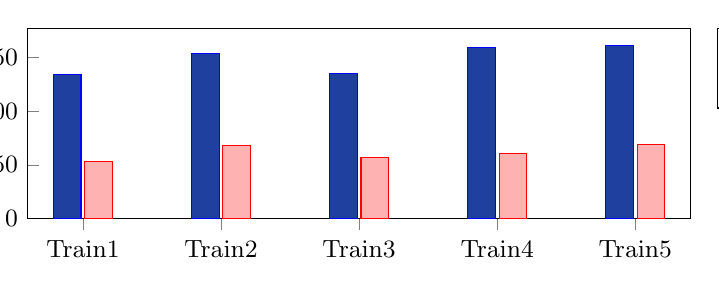
\begin{tikzpicture}[trim axis left, trim axis right]
	\begin{axis}[
	ybar,
	area legend,
	tick label style={font=\small},
	tickpos=left,
	xticklabels={Train1, Train2, Train3, Train4, Train5}, 
	xtick={1,2,3,4,5},
	ymin=0,
	legend entries={BsAs,Cba},
	legend style={at={(1.04,1.002)}, anchor=north west,draw=black}, 
	]
	\addplot +[bar shift=-.2cm, area legend, fill={rgb:red,1;green,2;blue,5}] coordinates {(1,134) (2,154) (3,135) (4,159) (5,161)};
	
	\addplot  +[bar shift=.2cm, area legend]coordinates {(1,53) (2,68) (3,57) (4,61) (5,69)};
	\end{axis}
	\end{tikzpicture}
\end{figure}

\begin{figure}[H]
	\centering
	\pgfplotsset{width=10cm, height=4cm}
	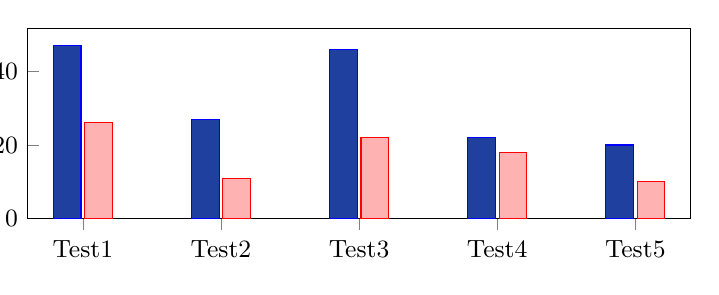
\begin{tikzpicture}[trim axis left, trim axis right]
	\begin{axis}[
	ybar,
	tick label style={font=\small},
	tickpos=left,
	xticklabels={Test1, Test2, Test3, Test4, Test5}, 
	xtick={1,2,3,4,5},
	ymin=0,
	]
	\addplot +[bar shift=-.2cm, area legend, fill={rgb:red,1;green,2;blue,5}] coordinates {(1,47) (2,27) (3,46) (4,22) (5,20)};
	
	\addplot  +[bar shift=.2cm, area legend]coordinates {(1,26) (2,11) (3,22) (4,18) (5,10)};
	\end{axis}
	\end{tikzpicture}
	\caption{Cantidad de instancias de Buenos Aires y Córdoba según cada grupo de Train y Tests}
	\label{TestsInstances}
\end{figure}

La tabla \ref{class_corr_en_pct} resume los resultados de clasificación correcta (en porcentaje) para los distintos clasificadores.

\begin{table}[H]
	\centering
	\begin{tabular}{|l|c|c|c|c|c|c|}
		\hline
		\textbf{}  & \textbf{Zero Rule} & \textbf{Ripper} & \textbf{C4.5} & \textbf{SVM} & \textbf{NaiveBayes} \\ \hline
		\textbf{Fold 1}  & 64 & 61 & 64 & 73 & 63 \\ \hline
		\textbf{Fold 2}  & 71 & 68 & 71 & 76 & 71 \\ \hline
		\textbf{Fold 3}  & 67 & 54 & 45 & 75 & 67 \\ \hline
		\textbf{Fold 4}  & 55 & 52 & 55 & 67 & 80 \\ \hline
		\textbf{Fold 5}  & 66 & 70 & 66 & 70 & 70 \\ \hline
		\hline \hline
		\textbf{Promedio} & 64 & 61 & 60 & 72 & 70 \\ \hline
	\end{tabular}
	\caption{Clasificación correcta en porcentaje}
	\label{class_corr_en_pct}
\end{table}

En esta tabla, Fold 1 corresponde al primer par $<$train, test$>$, Fold 2 al segundo par y así sucesivamente. En la Figura \ref{porcentajexClasificador} se puede ver gráficamente los resultados de clasificación correcta de dicha tabla. Excluimos a Ripper y C4.5 por dar muy parecido a Zero Rule.

\begin{figure}[H]
	\centering
	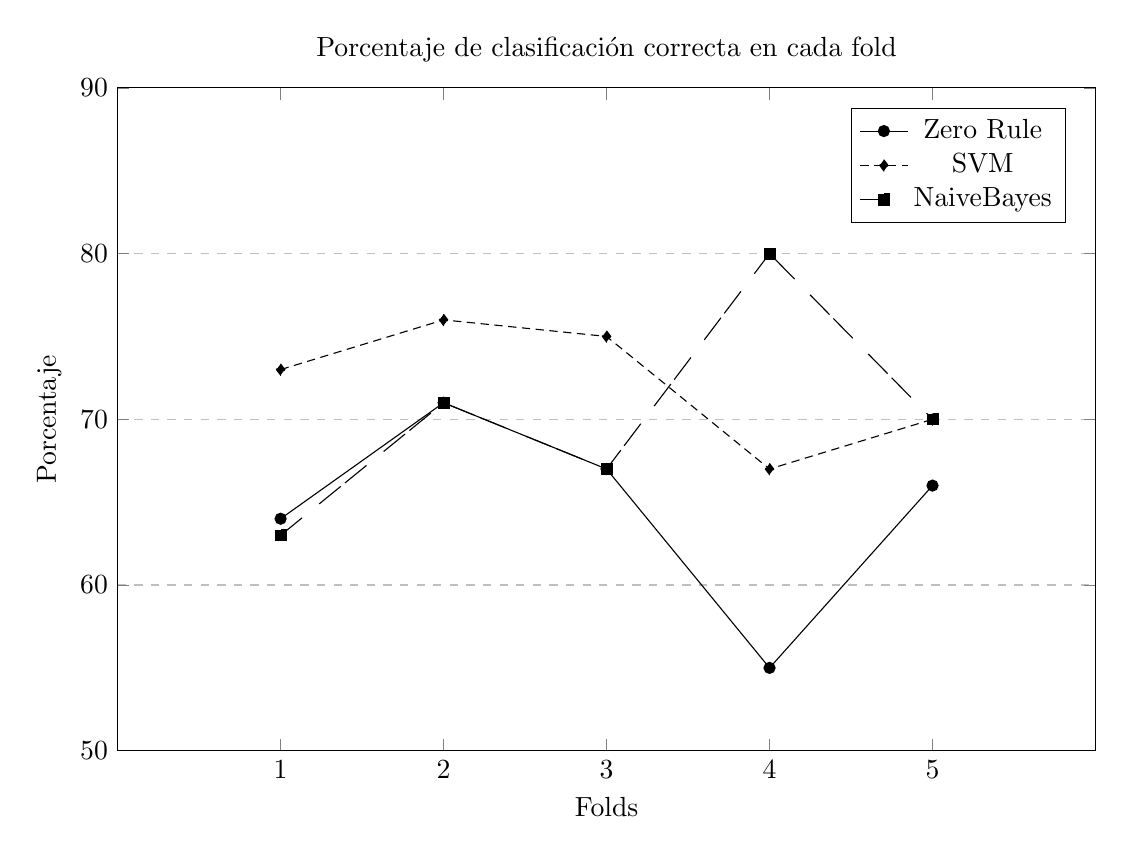
\begin{tikzpicture}
	\begin{axis}[
	width=14cm,
	height=10cm,
	title={Porcentaje de clasificación correcta en cada fold},
	xlabel={Folds},
	ylabel={Porcentaje},
	xmin=0, xmax=6,
	ymin=50, ymax=90,
	xtick={1,2,3,4,5},
	ytick={20,30,40,50,60,70,80,90,100},
	legend pos=north east,
	ymajorgrids=true,
	grid style=dashed
	] 
	\addplot [mark=otimes*, width=1pt] coordinates {
		(1,64)(2,71)(3,67)(4,55)(5,66) };\addlegendentry{Zero Rule};
	%\addplot[mark=diamond*,dash pattern=on 10pt off 2pt on 3pt off 2pt]coordinates {
	%    (1,61)(2,68)(3,54)(4,52)(5,70) };\addlegendentry{JRip};
	\addplot [mark=diamond*,dash pattern=on 3pt off 2pt on 3pt off 2pt]coordinates {
		(1,73)(2,76)(3,75)(4,67)(5,70) };\addlegendentry{SVM};
	\addplot [mark=square*,dash pattern=on 10pt off 8pt on 10pt off 2pt]coordinates {
		(1,63)(2,71)(3,67)(4,80)(5,70) };\addlegendentry{NaiveBayes};
	\end{axis}
	\end{tikzpicture}
	\caption{Porcentaje de Zero Rule, SVM y NaiveBayes}
	\label{porcentajexClasificador}
\end{figure}

Recordemos que el clasificador Zero Rule elige siempre la clase mayoritaria en su grupo de test. Viendo la Figura \ref{porcentajexClasificador} podemos notar que Zero Rule mantiene un porcentaje en los diferentes tests entre un 55\% y casi 70\%. El clasificador Support vector machine (SVM) siempre se mantiene por arriba de este Baseline.

Algo interesante sucede con el clasificador NaiveBayes: muestra resultados muy similares a Zero Rule pero en el test 4 posee mucha mejor performance. Viendo los grupos generados en la Figura \ref{TestsInstances}, el fold 4 es el que tiene menos diferencia entre cantidad de hablantes de Buenos Aires y Córdoba. Al tener mitad instancias de cada grupo y como Zero Rule elige entre uno de esos dos, va a poseer un porcentaje de acierto cercano al 50\%, como sucede.  

El porcentaje de exactitud en la clasificación se puede apreciar con las métricas \textit{Precision} y \textit{Recall}. \textit{Precision} se define como la cantidad de verdaderos positivos sobre la cantidad de verdaderos y falsos positivos. \textit{Recall} se define como la cantidad de verdaderos positivos sobre la cantidad de verdaderos positivos y falsos negativos. Tomamos como verdaderos positivos a la condición de que fue clasificado como Buenos Aires y efectivamente es de ahí. Falsos negativos si el hablante es de Buenos Aires pero es clasificado como Córdoba. Y falso positivo si el hablante es de Córdoba pero es clasificado como Buenos Aires. 

%http://en.wikipedia.org/wiki/Precision_and_recall

Las Figuras \ref{ZeroR_matrizconf}, \ref{FSMO_matrizconf} y \ref{NaiveBayes_matrizconf} muestran los valores que  surgen de la matriz de confusión. Vamos a analizar como son estas métricas para el caso del test 4, que es el más interesante.

% Precision = VP / VP + FP
% Recall = VP / VP + FN
% VP = "BsAs classif. como BsAs"
% FN = "BsAs classif. como Cba"
% FP = "Cba classif. como BsAs" 

%\begin{center}
%\Large Matrices de confusión para test 4
%\end{center}

\begin{figure}[H]
	\centering
	\paragraph*{Zero Rule:}\mbox{}\\
	\begin{table}[H]
		\centering
		\begin{tabular}{|c|c|l|c|c|c|c|}
			\hline
			BsAs & Cba &  \\ \hline
			22 &  18 &  Clasificado como BsAs \\ \hline
			0  &   0 &  Clasificado como Cba \\ \hline
		\end{tabular}
	\end{table}
	\begin{center}
		\textbf{Precision = 22/40 = 0.55;} \textbf{Recall = 1}\\
		\textbf{Instancias correctas = 55\%}
	\end{center}
	\caption{Matriz de confusión para Zero Rule en el test 4}
	\label{ZeroR_matrizconf}
\end{figure}

\begin{figure}[H]
	\centering
	\paragraph*{Support vector machine:}\mbox{}\\
	\begin{table}[H]
		\centering
		\begin{tabular}{|c|c|l|c|c|c|c|}
			\hline
			BsAs & Cba &  \\ \hline
			22 &  13 &  Clasificado como BsAs \\ \hline
			0  &   5 &  Clasificado como Cba \\ \hline
		\end{tabular}
	\end{table}
	\begin{center}
		\textbf{Precision = 22/35 = 0.63;} \textbf{Recall = 1}\\
		\textbf{Instancias correctas = 67\%}
	\end{center}
	\caption{Matriz de confusión para SVM en el test 4}
	\label{FSMO_matrizconf}
\end{figure}

\begin{figure}[H]
	\centering
	\paragraph*{NaiveBayes:}\mbox{}\\
	\begin{table}[H]
		\centering
		\begin{tabular}{|c|c|l|c|c|c|c|}
			\hline
			BsAs & Cba &  \\ \hline
			20 &  6 &  Clasificado como BsAs \\ \hline
			2  &  12 &  Clasificado como Cba \\ \hline
		\end{tabular}
	\end{table}
	\begin{center}
		\textbf{Precision = 20/26 = 0.77;} \textbf{Recall = 20/22 = 0.9}\\
		\textbf{Instancias correctas = 80\%}
	\end{center}
	\caption{Matriz de confusión para NaiveBayes en el test 4}
	\label{NaiveBayes_matrizconf}
\end{figure}

Viendo estas matrices de confusión y sus métricas podemos observar cuál es el error que se produce en cada uno de los clasificadores. Notamos que Zero Rule produce mucho \textit{Error de tipo I} (clasificador afirma que es de Buenos Aires y en realidad es de Córdoba). Esto sucede ya que elige sólo una categoría siempre. En los demás clasificadores se intenta realmente predecir y por eso los Errores de tipo I y II están más distribuidos.

Otro dato a tener en cuenta es que, si bien el clasificador Zero Rule tuvo un valor alto en la métrica \textit{Recall}, no fue lo mismo para \textit{Precision} y por eso el valor de instancias correctas dio bastante malo. Ambos valores deben estar cercanos al 1 para tener una buena performance. Por eso en el caso de NaiveBayes; si bien ningún valor dio 1, ambos están cerca y posee en mayor porcentaje de instancias correctas.

Puede suceder que el porcentaje de instancias correctas sea el mismo pero los Errores de tipo I y II sean más balanceados. Esto es el caso del conjunto de test 1. Las tablas de las Figuras \ref{ZeroR_matrizconf_2}, \ref{NaiveBayes_matrizconf_2} muestran este caso para los clasificadores Zero Rule y NaiveBayes.

%\begin{center}
%\Large Matrices de confusión para test 1
%\end{center}

\begin{figure}[H]
	\centering
	\paragraph*{Zero Rule:}\mbox{}\\
	\begin{table}[H]
		\centering
		\begin{tabular}{|c|c|l|c|c|c|c|}
			\hline
			BsAs & Cba &  \\ \hline
			47 &  26 &  Clasificado como BsAs \\ \hline
			0 &  0 &  Clasificado como Cba \\ \hline
		\end{tabular}
	\end{table}
	\begin{center}
		\textbf{Precision = 47/73 = 0.64;} \textbf{Recall = 47/47 = 1}\\
		\textbf{Instancias correctas = 64\%}
	\end{center}
	\caption{Matriz de confusión para Zero Rule en el test 1}
	\label{ZeroR_matrizconf_2}
\end{figure}

\begin{figure}[H]
	\centering
	\paragraph*{NaiveBayes:}\mbox{}\\
	\begin{table}[H]
		\centering
		\begin{tabular}{|c|c|l|c|c|c|c|}
			\hline
			BsAs & Cba &  \\ \hline
			33 &  13 &  Clasificado como BsAs \\ \hline
			14 &  13 &  Clasificado como Cba \\ \hline
		\end{tabular}
	\end{table}
	\begin{center}
		\textbf{Precision = 33/46 = 0.7;} \textbf{Recall = 33/47 = 0.7}\\
		\textbf{Instancias correctas = 63\%}
	\end{center}
	\caption{Matriz de confusión para NavieBayes en el test 1}
	\label{NaiveBayes_matrizconf_2}
\end{figure}

En este caso notamos que, a pesar de que el porcentaje de instancias correctas den valores cercanos, Zero Rule concentra gran parte del error en un tipo sólo, mientras que NaiveBayes lo distribuye entre los dos tipos.

No realizaremos los tests estadísticos de Wilcoxon y Test t de Student para este modelo de test. La razón es que los conjuntos de test de cada fold no son independientes. Recordemos que tienen 20 \% de instancias repetidas, entonces cada fold por separado no es estadísticamente independiente. Es por ello que dejamos de lado los tests estadísticos.

%\subsection{Wilcoxon y Test t de Student}
%
%En esta sección mostramos los resultados de estos tests estadísticos. Recordemos que los resultados surgieron de realizar los test de Wilcoxon y t de Student para el vector resultado de cada clasificador con respecto a ZeroR. Los resultados expresados en p-valor se pueden observar en la tabla \ref{res_tests_wilcoxon_student}.
%
%\begin{table}[H]
%	\centering
%	\begin{tabular}{|l|c|c|c|c|c|c|}
%		\hline
%		\textbf{}  & \textbf{Student Test} & \textbf{Wilcoxon Test} \\ \hline
%		\textbf{ZeroR y JRip}  & 0.8438 & 0.87 \\ \hline
%		\textbf{ZeroR y J48}  & 0.9772 & 0.813 \\ \hline
%		\textbf{ZeroR y NaiveBayes}  & 0.2113 & 0.1692 \\ \hline
%		\textbf{ZeroR y Function SMO}  & 0.03125 & 0.004545 \\ \hline
%	\end{tabular}
%	\caption{Resultados de cada test representado en p-valor}
%	\label{res_tests_wilcoxon_student}
%\end{table}
%
%Todos los clasificadores pasaron el test Shapiro-Wilk, entonces podemos afirmar que los resultados de cada clasificador corresponden a una distribución Normal. Analizando los resultados resumidos en la Figura \ref{res_tests_wilcoxon_student} notamos que para el clasificador Function SMO posee p-valor menor a 0,05 en ambas columnas. Esto quiere decir que para \textbf{Function SMO hay evidencia suficiente de ser mejor que ZeroR}. Por otro lado, los demás no pudieron lograr este cometido. 

\subsubsection{Análisis de los clasificadores construidos}

Analizamos los clasificadores construidos para cada fold. Estos nos dan más información para entender los resultados. Notamos que los clasificadores Support vector machine y NaiveBayes utilizaron todos los atributos para su clasificación. Fueron los que más provecho sacaron a los atributos. Por otro lado, el clasificador C4.5 armó un árbol de decisión sólo de un nivel. Es por esto que tuvo una mala performance y no aprovechó los atributos.

Para analizar mas en profundidad, veamos la salida del clasificador Ripper ya que, de los clasificadores elegidos, es el que nos provee reglas utilizando una cantidad pequeña de atributos que podemos analizar en este trabajo.

Cada uno de los folds devolvió un conjunto de reglas y no fueron necesariamente iguales entre sí. Estos datos corresponden a la clasificación para fold 1.

\begin{flushleft}
	\begin{itemize}
		
		\item $(FON\_ll\_norm <= -11.08) and (ACU\_AverageLL\_6 <= 4.308) => place=cba (12.0/0.0)$ \\
		\item $(FON\_Sfinal\_normhd <= 27.874) and (SIL\_prevSyllableAccent\_norm >= -4.265) => place=cba (11.0/1.0)$ \\
		\item $(FON\_rr\_normhd <= 31.355) => place=cba (10.0/2.0)$ \\
		\item $ else  => place=bsas (154.0/23.0)$
	\end{itemize}
\end{flushleft}

En esta regla; la duración sobre /ll/, el estiramiento de la /s/ al final de la palabra, la duración sobre /r/ y la duración de la sílaba anterior a la acentuada fueron los elegidos para clasificar los dos grupos. Si bien este clasificador no obtuvo buena performance, analizar sus reglas nos permite pensar cuáles atributos tienen mayor importancia a la hora de la clasificación.

\subsubsection{Características del modelo de test}

Analizando los resultados de la tabla \ref{class_corr_en_pct} y las características de cada fold encontramos los siguientes problemas.
%En esta sección vamos a analizar los datos que obtuvimos en este cross-validation. Para ello analizamos los valores de la Tabla \ref{class_corr_en_pct} y las características del armado de cada fold. Las características son:

\begin{itemize}
	\item \textbf{Los grupos de tests no son independientes:} Si tomamos dos tests al azar de esta validación cruzada sucede que tiene instancias de audios repetidas. Esto es una característica que intentaremos evitar en los próximos modelos de test.
	
	\item \textbf{El clasificador C4.5 tiene el mismo rendimiento que Zero Rule:} Si vemos el promedio de porcentajes clasificados correctamente y lo comparamos con Zero Rule vemos que inclusive es menor. Viendo el clasificador creado por C4.5 notamos que, en todos los folds, armaba árboles de sólo un nodo de altura. 
	
	\item \textbf{Zero Rule tiene un rendimiento mejor al 50 \%: } Este clasificador elige siempre la clase mayoritaria. Si su rendimiento es mayor al 50 \% quiere decir que hay más instancias de una clase que de otra. Particularmente, hay más instancias de Buenos Aires que de Córdoba.
\end{itemize}

En los siguiente modelos de test intentamos mejorar estos problemas.



%nuevos
% Un hablante para test, lo demás para train
%\subsection{Un hablante para test y los demás para train}
\subsection{Clasificación por muestra}
\label{un_hablante_para_test_los_demas_train}

\usetikzlibrary{shapes.geometric}

\tikzset{myshade/.style={minimum size=.4cm,shading=radial,inner color=white,outer color={#1!90!gray}}}
\newcommand\mycirc[1][]{\tikz\node[circle,myshade=#1]{};}

Definimos un modelo de test donde enfatizamos la idea de  distinguir un hablante. Para cada fold generado, excluiremos un hablante y entrenaremos con todos los demás. Luego testeamos contra ese hablante excluido. Este esquema evita que tengamos grabaciones repetidas en los grupos de tests. Podemos ver este esquema en la tabla \ref{HPTDT_esq_cv}. También es conocido como \textbf{validación cruzada dejando uno fuera} (en inglés: Leave-one-out cross-validation)

En nuestro conjunto de datos tenemos 27 hablantes: 19 de Buenos Aires y 8 de Córdoba. Vamos a tener 27 folds distintos para cada uno de ellos. Cada uno de estos folds va a excluir todos los audios de este hablante, por eso cuando nos referimos a un hablante nos referimos a todos los audios grabados por él.

\begin{center}
	\mycirc[blue] Hablante para train \mycirc[red] Hablante para test
\end{center}

\begin{table}[H]
	\centering
	\begin{tabular}{cccccccccccc}
		& \multicolumn{11}{c}{\textit{Número de hablante}} \\
		& 1 & 2 & 3 & 4 & 5 & 6 & 7 & ... & 25 & 26 & 27 \\
		\hline \\
		Fold 1 &\mycirc[red] & \mycirc[blue] & \mycirc[blue]  & \mycirc[blue]  & \mycirc[blue]  & \mycirc[blue]  & \mycirc[blue] & ... & \mycirc[blue] & \mycirc[blue] & \mycirc[blue]  \\
		
		Fold 2 &\mycirc[blue] & \mycirc[red] & \mycirc[blue]  & \mycirc[blue]  & \mycirc[blue]  & \mycirc[blue]  & \mycirc[blue] & ... & \mycirc[blue] & \mycirc[blue] & \mycirc[blue]  \\
		
		Fold 3 &\mycirc[blue] & \mycirc[blue] & \mycirc[red]  & \mycirc[blue]  & \mycirc[blue]  & \mycirc[blue]  & \mycirc[blue] & ... & \mycirc[blue] & \mycirc[blue] & \mycirc[blue]  \\
	
		\multicolumn{11}{c}{\textit{...}}	\\
		
		Fold 27 &\mycirc[blue] & \mycirc[blue] & \mycirc[blue]  & \mycirc[blue]  & \mycirc[blue]  & \mycirc[blue]  & \mycirc[blue] & ... & \mycirc[blue] & \mycirc[blue] & \mycirc[red]   \\
	
	\end{tabular}
	\caption{Esquema de validación cruzada}
	\label{HPTDT_esq_cv}
\end{table}
		
\subsubsection{Resultados}

En la tabla \ref{HPTDT_clas_xval_porHab} podemos observar los resultados de clasificación. No resulta relevante mostrar el porcentaje de clasificación correcta para cada fold. Expresamos el promedio de clasificación correcta de cada fold para cada clasificador como se muestra en la siguiente fórmula.

\textbf{Promedio de porcentaje correcto en cada fold:}
\[
{ \sum_{i=1}^{\text{\# de folds}} \text{Porcentaje instancias correctas en fold \textit{i}}
	\over
	\text{\# de folds}
}
\]

\begin{table}[H]
	\centering
	\begin{tabular}{|l|c|c|c|c|c|c|}
		\hline
		\textbf{}  & \textbf{Zero Rule} & \textbf{Ripper} & \textbf{C4.5} & \textbf{SVM} & \textbf{NaiveBayes} \\ \hline
		%\textbf{Fold 1}  &  &  &  &  &  \\ \hline
		%\hline \hline
		\textbf{Promedio} & 70.37  & 69.47 & 70.37 & 71.34 & 71.46 \\ \hline
	\end{tabular}
	\caption{Clasificación correcta en porcentaje}
	\label{HPTDT_clas_xval_porHab}
\end{table}

Llama la atención que todos los clasificadores tuvieron porcentajes muy cercanos. Esto lo analizaremos más adelante. 

Realizamos los test estadísticos de Wilcoxon y Test t de Student para este modelo de test. En este caso, las muestras de test son independientes entre sí. Estos resultados se pueden observar en la tabla  \ref{HPTDT_res_tests_wilcoxon_student}.

\begin{table}[H]
	\centering
	\begin{tabular}{|l|c|c|c|c|c|c|}
		\hline
		\textbf{}  & \textbf{Student Test} & \textbf{Wilcoxon Test} \\ \hline
		\textbf{ZeroR y Ripper}  & 0.5816 & 0.6234 \\ \hline
		\textbf{ZeroR y C4.5}  & 1 & 1 \\ \hline
		\textbf{ZeroR y NaiveBayes}  & 0.4383 & 0.4042 \\ \hline
		\textbf{ZeroR y SVM}  & 0.4302 & 0.2646 \\ \hline
	\end{tabular}
	\caption{Resultados de cada test representado en p-valor}
	\label{HPTDT_res_tests_wilcoxon_student}
\end{table}

Los valores expresados corresponden al p-valor. Todos los clasificadores pasaron el test Shapiro-Wilk, entonces podemos afirmar que los resultados de cada clasificador corresponden a una distribución Normal. A pesar de esto, realizamos ambos tests estadísticos para cada uno. Estos test mostraron que las diferencias entre cada clasificador y el baseline no son estadísticamente significativos.

Recordemos que no todos los hablantes aportaron igual cantidad de grabaciones. Ellos tenían la opción de seguir aportando grabaciones o salir de la aplicación. Es por esto que cada porcentaje de fold no aporta igual cantidad de instancias correctas. Por ejemplo: puede suceder que la cantidad de instancias para un fold es $1$ y si esa muestra fue correctamente clasificada el porcentaje de instancias correctas dará $100\%$. Mientras que otro fold puede tener $10$ instancias y clasificar correctamente $9$ concluyendo que su porcentaje de instancias correctas dará $90\%$. En la figura \ref{CantDeMuestrasXcadaTest} podemos ver la cantidad de grabaciones en cada grupo de testeo. 

\begin{figure}[H]
	\centering
	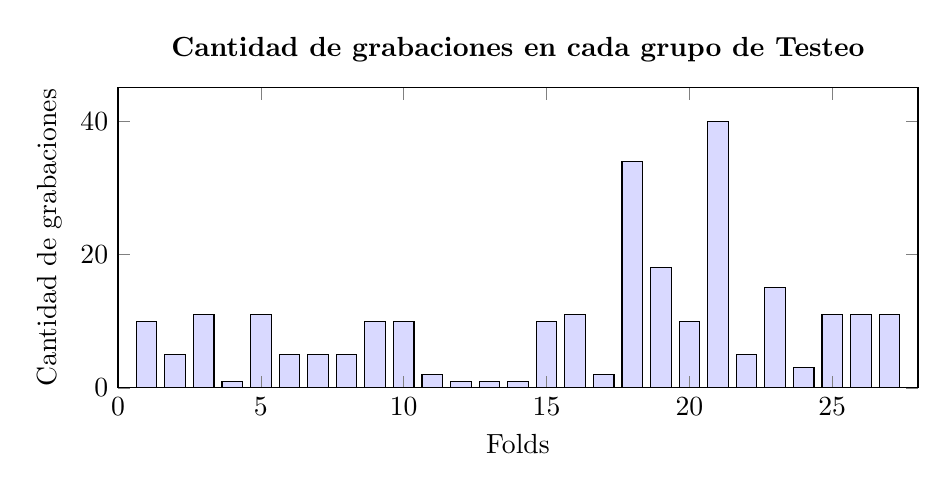
\begin{tikzpicture}
	
	\begin{axis}[
	title={\textbf{Cantidad de grabaciones en cada grupo de Testeo}},
	xlabel={Folds},
	ylabel={Cantidad de grabaciones},
	scale only axis,
	width=4in,
	height=1.5in,
	xmin=0, xmax=28,
	ymin=0, ymax=45,
	axis on top]
	\addplot[
	ybar,
	fill=blue!15,
	bar width=0.102874in, 
	bar shift=0in,
	draw=black] 
	plot coordinates{ 
		(1, 10)(2, 5)(3, 11)(4, 1)(5, 11)(6, 5)(7, 5)(8, 5)(9, 10)(10,10)(11,2)(12,1)(13,1)(14,1)(15,10)(16,11)(17,2)(18,34)(19,18)(20,10)(21,40)(22,5)(23,15)(24,3)(25,11)(26,11)(27,11) 
	};
	
	\end{axis}
	\end{tikzpicture}	
	\caption{Cantidad de muestras para cada Test}
	\label{CantDeMuestrasXcadaTest}
\end{figure}

Debemos tener una mejor métrica para equiparar la cantidad de instancias correctas en cada fold. Para evitar promediar por porcentaje correcto en cada grupo de test, realizamos el promedio sumando la cantidad de instancias correctas. Los resultados de cada clasificador utilizando esta nueva métrica se pueden ver en la figura\ref{HPTDT_clas_xval_porHab}. La fórmula calculada para cada clasificador se puede ver a continuación:

\textbf{Promedio de instancias correctas sobre instancias totales:}
\small
\[
{ \sum_{i=1}^{\text{\# de folds}} \text{Cantidad de instancias correctas en fold \textit{i}}
	\over
	\text{\# de instancias}
}
\]

{\small 	
\begin{table}[H]
	\centering
	\begin{tabular}{|l|c|c|c|c|c|c|}
		\hline
		\textbf{}  & \textbf{Zero Rule} & \textbf{Ripper} & \textbf{C4.5} & \textbf{SVM} & \textbf{NaiveBayes} \\ \hline
		%\textbf{Fold 1}  &  &  &  &  &  \\ \hline
		%\hline \hline
		\textbf{Promedio} & 69  & 63 & 69 & 70 & 65 \\ \hline
	\end{tabular}
	\caption{Clasificación correcta en cantidad de instancias}
	\label{HPTDT_clas_xval_porHab}
\end{table}}

Notamos que los resultados varían algunos puntos pero no a grandes rasgos. El clasificador que más varia es NaiveBayes con casi $5\%$ menos. A pesar de ello, no parece cambiar mucho el promedio de cada clasificador.
	



\subsubsection{Análisis de los clasificadores construidos}

Analizamos los clasificadores armados para cada fold. El clasificador Ripper generó reglas utilizando un conjunto acotado de atributos. En cambio, los clasificadores Support vector machine y NaiveBayes utilizaron todos los atributos ponderando cada uno por valores escalares. El clasificador C4.5 tuvo también una performance pobre por tener un árbol de un nivel solo.  

Podemos ver el conjunto de reglas que generó el clasificador Ripper para el fold 4:

\begin{flushleft}
	\begin{itemize}
		\item $(FON\_rr\_norm <= -6.901) and (ACU\_AverageRR\_7 <= 11.23) => place=cba (18.0/3.0)$ \\
		\item $(FON\_ll\_norm <= -7.975) and (ACU\_AverageLL\_6 <= 4.308) => place=cba (15.0/0.0)$
		\item $else => place=bsas (222.0/49.0)$
	\end{itemize}
\end{flushleft}

Notamos que sigue utilizando los atributos temporales y en menor medida los atributos acústicos.

A continuación, podemos ver el Árbol de decisión generado por C4.5 para cada fold. 

\dirtree{%
	.1 root.
	.2 $bsas (249.0/68.0)$.
}

Al armar un árbol de decisión de una sola rama y que siempre elige Buenos Aires, este clasificador elige de igual manera que ZeroRule. Por ende, ambos tienen igual performance.

\subsubsection{Características del modelo de test}

%El clasificador ZeroRule tiene muy buen rendimiento solamente por tener un conjunto de datos desequilibrado. También el clasificador C4.5 posee muy baja performance y su árbol de clasificación sigue siendo muy pobre.  

Analizando los distintos clasificadores, nos llama la atención que C4.5 obtuvo igual performance que ZeroRule. El clasificador C4.5 no saca provecho de los datos y termina creando un árbol de decisión eligiendo la clase mayoritaria.

Recordemos que el algoritmo C4.5 arma el árbol de decisión teniendo en cuenta la ganancia de información. Calcula esta métrica para cada atributo y el mayor de todos ellos se agrega como raíz del árbol. Luego descarta el atributo ya elegido y se llama recursivamente en cada rama. 

A simple vista, el clasificador no tiene problemas al utilizar atributos indefinidos. Al calcular para cada atributo su ganancia de información estaría descartando estos atributos. Pensamos que los parámetros utilizados generan demasiado \textit{prunning} en el árbol de decisión y termina quedando solamente una rama. Creemos que variando los parámetros se podría mejorar este árbol. Dejamos esta opción como trabajo futuro.

%Ver bien el mail de Miguel
%versión vieja
%Analizando el algoritmo del clasificador C4.5 notamos que el árbol generado puede ser muy pobre si en sus datos de entrenamiento hay muchos valores desconocidos. 

%Recordemos que el algoritmo C4.5 para armar el árbol de clasificación va tomando el atributo con mayor ganancia de información y agregándolo como un nuevo nodo al árbol. Luego descarta el atributo ya elegido y se llama recursivamente en cada rama. 

%Si hay muchas instancias con atributos desconocidos, pocos atributos tendrán buena ganancia de información y no podrá armar un árbol extenso. Recordemos que, para un hablante, cada uno de sus audios sólo define atributos para la frase grabada. Si en la grabación no se extrae ese atributo, quedará con valor desconocido. 

%\begin{table}[H]
%	\centering
%	\begin{tabular}{|l|l|ccccccccc|}
%		\hline
%		\multicolumn{2}{|l|}{Atributos} & A1 & A2 & A3 & A4 & A5 & A6 & A7 & ... & AN \\
%		\hline 
%		\textbf{Hablante 1} & \textbf{Audio1} & 1 & 2 & ? & ? & ? & ? & ? & ... & 2 \\
%		& \textbf{Audio2} & ? & ? & 1 & 3 & 4 & ? & ? & ... & ? \\
%		& \textbf{Audio3} & ? & ? & ? & ? & ? & 4 & 2 &  ... & ? \\
%		\hline
%	\end{tabular}
%	\caption{Ejemplo de atributos para un hablante}
%	\label{HPTDT_hablante_ej}
%\end{table}

%Veamos un ejemplo: en la tabla \ref{HPTDT_hablante_ej} podemos ver los atributos extraídos de un hablante ficticio. Supongamos que este hablante grabó sólo 3 audios. En el primer audio se define los atributos A1, A2 y AN. En el segundo audio se define A3, A4 y A5. En último audio se define los atributos A6 y A7. Todos los demás atributos poseen valores desconocidos, pero en realidad corresponden a un mismo hablante. Si bien, para ese audio en particular es un atributo desconocido, la realidad es que corresponde a un mismo hablante y podemos inferirlo de otro audio grabado por él. Deberíamos tener alguna forma de evitar tener valores desconocidos cuando pueden ser extraídos de otro audio.

%Suponemos que el mal rendimiento de C4.5 viene de la mano de los valores desconocidos. Creemos que si tenemos menor cantidad de valores desconocidos esta performance mejorará. Pensamos esta idea luego de leer cómo funciona los árboles de decisión del libro \cite{DataMining-PracticalMachineLearningTools} \footnote{En la página 194 está la explicación que nos ayudó a razonar esta idea.}. En la sección \ref{prom_los_atributos_de_cada_hablante} probaremos otro modelo de test que intente evitar tener tantos valores desconocidos. 


% % % % % % % % % % % % % % % % % % % % % % % % % % % % % % % % % %
% Correcciones a agregar
%Correcciones a agregar
%
%
%\begin{center}
%	\begin{tikzpicture}
%	
%	\begin{axis}[
%	title={\textbf{Cantidad de grabaciones en cada grupo de Testeo}},
%	xlabel={Folds},
%	ylabel={Cantidad de grabaciones},
%	scale only axis,
%	width=4in,
%	height=2in,
%	xmin=0, xmax=28,
%	ymin=0, ymax=45,
%	axis on top]
%	\addplot[
%	ybar,
%	fill=blue!15,
%	bar width=0.102874in, 
%	bar shift=0in,
%	draw=black] 
%	plot coordinates{ 
%		(1, 10)(2, 5)(3, 11)(4, 1)(5, 11)(6, 5)(7, 5)(8, 5)(9, 10)(10,10)(11,2)(12,1)(13,1)(14,1)(15,10)(16,11)(17,2)(18,34)(19,18)(20,10)(21,40)(22,5)(23,15)(24,3)(25,11)(26,11)(27,11) 
%	};
%	
%	\end{axis}
%	\end{tikzpicture}	
%\end{center}
%
%
%\textbf{Promedio de porcentaje correcto en cada fold:}
%\[
%{ \sum_{i=1}^{\text{\# de folds}} \text{Porcentaje instancias correctas en fold \textit{i}}
%	\over
%	\text{\# de folds}
%}
%\]
%
%{\small 	\begin{table}[H]
%		\centering
%		\begin{tabular}{|l|c|c|c|c|c|c|}
%			\hline
%			\textbf{}  & \textbf{Zero Rule} & \textbf{Ripper} & \textbf{C4.5} & \textbf{SVM} & \textbf{NaiveBayes} \\ \hline
%			%\textbf{Fold 1}  &  &  &  &  &  \\ \hline
%			%\hline \hline
%			\textbf{Promedio} & 70  & 69 & 70 & 71 & 71 \\ \hline
%		\end{tabular}
%		\caption{Clasificación correcta en porcentaje}
%		\label{HPTDT_clas_xval_porHab}
%	\end{table}}
%	
%	\textbf{Promedio de instancias correctas sobre instancias totales:}
%	\small
%	\[
%	{ \sum_{i=1}^{\text{\# de folds}} \text{Cantidad de instancias correctas en fold \textit{i}}
%		\over
%		\text{\# de instancias}
%	}
%	\]
%	
%	{\small 	\begin{table}[H]
%			\centering
%			\begin{tabular}{|l|c|c|c|c|c|c|}
%				\hline
%				\textbf{}  & \textbf{Zero Rule} & \textbf{Ripper} & \textbf{C4.5} & \textbf{SVM} & \textbf{NaiveBayes} \\ \hline
%				%\textbf{Fold 1}  &  &  &  &  &  \\ \hline
%				%\hline \hline
%				\textbf{Promedio} & 69  & 63 & 69 & 70 & 65 \\ \hline
%			\end{tabular}
%			\caption{Clasificación correcta en cantidad de instancias}
%			\label{HPTDT_clas_xval_porHab}
%		\end{table}}
%		
%		

% Juntar por cada hablante sus audios en una muestra sola promediando sus atributos
\subsection{Promediando los atributos de cada hablante}
\label{prom_los_atributos_de_cada_hablante}

Vamos a armarnos un modelo de test similar al anterior pero donde su conjunto de datos no sea desequilibrado con respecto a la cantidad de instancias de cada clase. Nunca es bueno descartar datos pero debemos tener un conjunto de datos equilibrado para saber si utilizando los atributos que definidos podemos realizar una mejor clasificación que el baseline.

Tomaremos 8 hablantes de Buenos Aires y de 8 Córdoba. De esta forma, el conjunto de datos está equilibrado en cantidad. La elección de cada uno de estos hablantes fue al azar. Como el esquema anterior, vamos a tener un fold por cada hablante. En la Tabla \ref{cv-porHabProm} vemos este esquema.

\begin{center}
	\mycirc[blue] Hablante para train \mycirc[red] Hablante para test
\end{center}

\begin{table}[H]
	\centering
	\begin{tabular}{cccccccccccc}
		& \multicolumn{11}{c}{\textit{Número de hablante}} \\
		& 1 & 2 & 3 & 4 & 5 & 6 & 7 & ... & 14 & 15 & 16 \\
		\hline \\
		Fold 1 &\mycirc[red] & \mycirc[blue] & \mycirc[blue]  & \mycirc[blue]  & \mycirc[blue]  & \mycirc[blue]  & \mycirc[blue] & ... & \mycirc[blue] & \mycirc[blue] & \mycirc[blue]  \\
		
		Fold 2 &\mycirc[blue] & \mycirc[red] & \mycirc[blue]  & \mycirc[blue]  & \mycirc[blue]  & \mycirc[blue]  & \mycirc[blue] & ... & \mycirc[blue] & \mycirc[blue] & \mycirc[blue]  \\
		
		Fold 3 &\mycirc[blue] & \mycirc[blue] & \mycirc[red]  & \mycirc[blue]  & \mycirc[blue]  & \mycirc[blue]  & \mycirc[blue] & ... & \mycirc[blue] & \mycirc[blue] & \mycirc[blue]  \\
		
		\multicolumn{11}{c}{\textit{...}}	\\
		
		Fold 16 &\mycirc[blue] & \mycirc[blue] & \mycirc[blue]  & \mycirc[blue]  & \mycirc[blue]  & \mycirc[blue]  & \mycirc[blue] & ... & \mycirc[blue] & \mycirc[blue] & \mycirc[red]   \\
		
	\end{tabular}
	\caption{Esquema de validación cruzada}
	\label{cv-porHabProm}
\end{table}

Otro problema que surgió de la validación cruzada anterior es la masiva cantidad de valores desconocidos. Pensamos que esto hace que clasificadores como C4.5 devuelvan resultados muy pobre. 

Para evitar esto realizamos lo siguiente: juntamos las grabaciones de cada hablante calculando su promedio para cada atributo. Veamos en la tabla \ref{datos_orig} un ejemplo de datos extraídos para entender la idea. 

\begin{table}[H]
	\centering
	\begin{tabular}{|l|l|ccccc|}
		\hline
		\multicolumn{2}{|l|}{Atributos} & A1 & A2 & A3 & ... & AN \\
		\hline 
		\textbf{Hablante 1} & \textbf{Audio1} & 1 & ? & 2 & & 2\\
		& \textbf{Audio2} & ? & ? & 1 & ... & ? \\
		& \textbf{Audio3} & 2 & ? & 3 & & ? \\
		\hline
		\textbf{Hablante 2} & \textbf{Audio1} & 1 & ? & ? & ... & ? \\
		& \textbf{Audio2} & 1 & 2 & ? & & ? \\
		\hline
	\end{tabular}
	\caption{Datos originales}
	\label{datos_orig}
\end{table}

Para cada hablante vamos a juntar sus audios realizando el promedio de cada atributo. Por ejemplo: el Hablante 1 grabó 3 audios donde cada uno posee distintos atributos. Juntamos todos esos audios en uno promediando sus atributos: El Audio1 y Audio3 poseen el atributo A1 con valor 1 y 2 respectivamente. Entonces en la tabla \ref{datos_comb} tendremos Audio1 con A1 definido como el promedio de estos valores: $1 + 2 = 1,5$. Ninguno de los audios grabados originalmente por Hablante 1 definió A2, entonces en este caso no vamos a poder definir ningún valor y va a quedar como valor desconocido. 

\begin{table}[H]
	\centering
	\begin{tabular}{|l|l|ccccc|}
		\hline
		\multicolumn{2}{|l|}{Atributos} & A1 & A2 & A3 & ... & AN \\
		\hline 
		\textbf{Hablante 1} & \textbf{Audio1} & \textbf{1.5} & \textbf{?} & \textbf{1.667} & ... & \textbf{2}\\
		\hline
		\textbf{Hablante 2} & \textbf{Audio1} & \textbf{1} & \textbf{2} & \textbf{?} & ... & \textbf{?} \\
		\hline
	\end{tabular}
	\caption{Atributos modificados}
	\label{datos_comb}
\end{table}

Resumiendo, por cada hablante se define una fila de atributos. Esto minimizaría la cantidad de valores desconocidos por cada grabación.

Esta variante la realizamos solamente utilizando los atributos temporales. Descartamos los atributos acústicos porque corresponden a grabaciones que en muchas oportunidades sufren de ruido y pensamos que también podía ser una causa por la cual los clasificadores tienen mal rendimiento.

\subsubsection{Resultados}

Los resultados de este cross-validaton podemos observarlo en la página \ref{class_corr_en_pct}.

\begin{table}[H]
	\centering
	\begin{tabular}{|l|c|c|c|c|c|c|}
		\hline
		\textbf{}  & \textbf{Zero Rule} & \textbf{Ripper} & \textbf{C4.5} & \textbf{SVM} & \textbf{NaiveBayes} \\ \hline
		\textbf{Promedio} & 53.33 & 60 & 60 & \textbf{93.33} & 80  \\ \hline
	\end{tabular}
	\caption{Clasificación correcta en porcentaje}
	\label{class_corr_en_pct}
\end{table}

Podemos observar que el clasificador Zero Rule estuvo más cerca de un valor esperable para el tipo de clasificador que es. Todos los demás dieron por arriba de este valor. Se destacaron los dos clasificadores que utilizan todos los atributos ponderados.

\subsubsection{Wilcoxon y Test t de Student}

Los resultados sobre el p-valor de cada test estadístico se puede ver en la tabla \ref{res_tests_wilcoxon_student}.

\begin{table}[H]
	\centering
	\begin{tabular}{|l|c|c|c|c|c|c|}
		\hline
		\textbf{}  & \textbf{Student Test} & \textbf{Wilcoxon Test} \\ \hline		
			\textbf{ZeroR y Ripper}  & 0.3351 & 0.3828 \\ \hline
			\textbf{ZeroR y C4.5}  & 0.2908 &  0.3864 \\ \hline
			\textbf{ZeroR y NaiveBayes}  & 0.05191 & 0.06472 \\ \hline
			\textbf{ZeroR y SVM}  &  \textbf{0.004282} & \textbf{0.009828} \\ \hline
	\end{tabular}
	\caption{Resultados de cada test representado en p-valor}
	\label{res_tests_wilcoxon_student}
\end{table}

Los clasificadores pasaron el test Shapiro-Wilk, entonces podemos afirmar que los resultados de cada clasificador corresponden a una distribución Normal y realizar el test T de Student.

Podemos observar que para el clasificador Support vector machines posee p-valor menor a 0,05 en ambas columnas. Esto quiere decir que para \textbf{Support vector machines hay evidencia suficiente de ser mejor que el baseline}. Por otro lado, los demás no pudieron lograr este cometido. 

\subsubsection{Clasificadores encontrados}

Analizando los clasificadores notamos que el clasificador C4.5 armó árboles de decisión más elaborados. Notamos eso también viendo que su performance superó a Zero Rules. 

Veamos un árbol de decisión generado por C4.5. Este corresponde al fold 7. 

\subsubsection*{Clasificador C4.5}

\dirtree{%
	.1 root.
	.2 $FON\_vowel\_norm <= 7.221824$.
	.3 $FON\_ll\_norm <= -24.007: cba (2.33/0.22)$.
	.3 $FON\_ll\_norm > -24.007: bsas (18.67/0.89)$.
	.2 $FON\_vowel\_norm > 7.221824: cba (5.0)$.
}
Los árboles de decisión generados esta vez utilizan mucho  atributos como $FON\_ll\_norm$ y $FON\_vowel\_norm$ en varios folds. Los demás clasificadores también armaron sus reglas: SVM y NaiveBayes ponderaron cada atributo para su clasificación mientras que Ripper armó sus reglas parecidas a C4.5. 

\subsubsection{Características del modelo de test}

Este modelo de test dió muy buenos resultados. El clasificador ZeroR tuvo una performance esperada de alrededor del 50 \% mientras que el clasificador C 4.5 pudo armar árboles mejores. 

Sin embargo, la forma que evitamos los valores desconocidos no es la mejor. El resultado de un fold para un determinado clasificador es 0\% o 100\%. Esto sucede porque es sólo una instancia la que representa. 

Esto también se ve reflejado en las matrices de confusión de cada fold. Cada una de ellas son de la forma: 

\begin{table}[H]
	\centering
	\begin{tabular}{|c|c|c|}
		\hline
		Buenos Aires & Córdoba & \\ \hline
		1 & 0 & Buenos Aires\\ \hline
		0 & 0 & Córdoba\\ \hline
	\end{tabular}
\end{table}

Donde siempre se encuentra sólo una instancia.


%% Cada hablante que tenga un atributo '?' cambiarlo por el promedio de ese atributo en las demás audios
\subsection{Promediando los atributos de cada hablante sólo si es desconocido}

En el anterior esquema vimos que promediando los atributo evitamos tener valores desconocidos. Sí bien esto es cierto, no es necesario promediar en todos los casos. 

Supongamos que tenemos el mismo conjunto de datos a la Tabla \ref{datos_orig}. Si para cada hablante promediamos sus atributos estaríamos perdiendo información. El hablante 1 tiene en el Audio1 el atributo A1 definido como 1, mientras que en el Audio3 como 2. Si realizáramos el promedio, estos valores específicos para estos audios los perderíamos.

%\begin{table}[H]
%	\centering
%	\begin{tabular}{|l|l|ccccc|}
%		\hline
%		\multicolumn{2}{|l|}{Atributos} & A1 & A2 & A3 & ... & AN \\
%		\hline 
%		\textbf{Hablante 1} & \textbf{Audio1} & 1 & ? & 2 & & 2\\
%		& \textbf{Audio2} & ? & ? & 1 & ... & ? \\
%		& \textbf{Audio3} & 2 & ? & 3 & & ? \\
%		\hline
%		\textbf{Hablante 2} & \textbf{Audio1} & 1 & ? & ? & ... & ? \\
%		& \textbf{Audio2} & 1 & 2 & ? & & ? \\
%		\hline
%	\end{tabular}
%	\caption{Atributos original}
%	\label{attr_orig}
%\end{table}

Es por ello que proponemos esta variante. Cuando haya un atributo desconocido en un audio, vamos a promediarlo con los atributos de los demás audios del mismo hablante. En la tabla \ref{attr_mod} se puede ver el resultado de esta variante marcado con negrita los nuevos valores. 

Por ejemplo: para el Hablante 1, el Audio1 no tiene definido el atributo A1. Entonces vamos a promediarlo con los demás audios. El Audio1 y Audio3 sí tienen este atributo definido y sus valores son 2 y 1 respectivamente. Realizamos el promedio nuevamente: $ 2 + 1 / 2 = 1,5$ entonces el valor del atributo 1 para el Audio2 es 1,5. De esta forma, no perdemos información con respecto al audio extraído.

\begin{table}[H]
	\centering
	\begin{tabular}{|l|l|ccccc|}
		\hline
		\multicolumn{2}{|l|}{Atributos} & A1 & A2 & A3 & ... & AN \\
		\hline 
		\textbf{Hablante 1} & \textbf{Audio1} & 1 & ? & 2 & & 2\\
		& \textbf{Audio2} & \textbf{1.5} & ? & 1 & ... & \textbf{2} \\
		& \textbf{Audio3} & 2 & ? & 3 & & \textbf{2} \\
		\hline
		\textbf{Hablante 2} & \textbf{Audio1} & 1 & \textbf{2} & ? & ... & ? \\
		& \textbf{Audio2} & 1 & 2 & ? & & ? \\
		\hline
	\end{tabular}
	\caption{Atributos modificados 2}
	\label{attr_mod}
\end{table}

Podemos observar los resultados del promedio de los folds para cada clasificador en la tabla \ref{class_corr_en_pct}. En este caso, el clasificador Zero Rule tuvo el porcentaje esperado y los demás por arriba de su valor. Esto nos muestra que utilizando estos atributos se puede superar el baseline. El clasificador que mejor performance tuvo fue Support vector machine.

\begin{table}[H]
	\centering
	\begin{tabular}{|l|c|c|c|c|c|c|}
		\hline
		\textbf{}  & \textbf{Zero Rule} & \textbf{Ripper} & \textbf{C4.5} & \textbf{SVM} & \textbf{NaiveBayes} \\ \hline
		\textbf{Promedio} & 50 & 72.44 & 73.48 & \textbf{77.19} & 74.62 \\ \hline
	\end{tabular}
	\caption{Clasificación correcta en porcentaje}
	\label{class_corr_en_pct}
\end{table}

\subsubsection{Wilcoxon y Test t de Student}

Los clasificadores pasaron el test Shapiro-Wilk. Gracias a esto podemos afirmar que los resultados de cada clasificador corresponden a una distribución Normal y podemos realizar el test de Student para todos ellos.

Corrimos los test estadísticos y obtuvimos que los resultados cada fold de NaiveBayes y Support vector machine tienen evidencia estadística para ser mejor que Zero rules. Podemos ver los p-valores en la tabla \ref{res_tests_wilcoxon_student}. Recordemos que para que tenga evidencia suficiente su p-valor debe ser menor a 0,05.

\begin{table}[H]
	\centering
	\begin{tabular}{|l|c|c|c|c|c|c|}
		\hline
		\textbf{}  & \textbf{Student Test} & \textbf{Wilcoxon Test} \\ \hline
		\textbf{ZeroR y Ripper}  & 0.06537 & 0.1284 \\ \hline
		\textbf{ZeroR y C4.5}  & 0.06156 &  0.1111 \\ \hline
		\textbf{ZeroR y NaiveBayes}  & \textbf{0.03916} & 0.06111 \\ \hline
		\textbf{ZeroR y SVM}  &  \textbf{0.02936} & \textbf{0.03522} \\ \hline
	\end{tabular}
	\caption{Resultados de cada test representado en p-valor}
	\label{res_tests_wilcoxon_student}
\end{table}

\subsubsection{Clasificadores encontrados}

Analizando los clasificadores para cada fold notamos que todos armaron clasificadores utilizando los atributos definidos. Como el modelo de test anterior, Support vector machine y NaiveBayes utilizaron todos los atributos mientras C4.5 y Ripper utilizaron reglas más simples.

\subsubsection{Características del modelo de test}

Con esta esquema mejoramos las matrices de confusión. La tabla \ref{mat_conf_f1} corresponde al primer fold. Notamos que ahora sí se analiza cada audio y se intenta clasificarlo. 

\begin{table}[H]
	\centering
	\begin{tabular}{|c|c|c|}
		\hline
		Buenos Aires & Córdoba & \\ \hline
		33 & 1 & Buenos Aires\\ \hline
		0 & 0 & Córdoba\\ \hline
	\end{tabular}
	\caption{Matriz de confusión fold 1}
	\label{mat_conf_f1}
\end{table}

% hablar de los problemas encontrados y cómo mejorarlos con el próximo cross-validation 


\section{Selección de atributos de forma automática}

%\subsection*{Attribute Evaluator: InfoGain}
%http://weka.sourceforge.net/doc.dev/weka/attributeSelection/InfoGainAttributeEval.html

%leer http://en.wikipedia.org/wiki/Information_gain_ratio

En esta sección aplicaremos evaluadores a los distintos atributos para analizar cuáles poseen mayor importancia. Para este análisis, utilizamos todo el conjunto de datos sin descartar ningún atributo. El evaluador utilizado fue la ganancia de información (InfoGain en Weka) para analizar la importancia de cada atributo. Utilizamos la opción Ranker que nos ordena los atributos de mayor a menor ganancia.

Estos algoritmos trabajan de la siguiente forma: para cada atributo calculan la entropía de la clase y luego se calcula la entropía de la misma sabiendo el valor de este atributo. La ganancia de información de ese atributo es la resta de esos dos resultados. Esto se puede expresar como: $InfoGain(Class,Attribute) = H(Class) - H(Class | Attribute)$. Veamos cada uno de estos términos.

\begin{itemize}
	\item $H(Class)$ representa el valor de la entropía de la clase a predecir. En otras palabras, mide la incertidumbre asociada a la clase sin tener en cuenta el valor de ningún atributo en particular. Recordemos que cuando decimos clase nos referimos a Buenos Aires o Córdoba.
	
	\item  $H(Class | Attribute)$ representa el valor de la entropía de la clase sabiendo el valor del atributo $Attribute$. A esta se le llama \textit{entropía condicional}. Si este atributo tiene información que ayude a predecir la clase, entonces la entropía condicional será menor a la entropía de la clase. O sea, $H(Class | Attribute) < H(Class)$. Cuanto menor sea la entropía condicional con respecto a la entropía de la clase, mayor será la ganancia de información para ese atributo.
\end{itemize}

La tabla \ref{infogain-table} nos muestra que los más preponderantes se refieren a la duración de consonantes (utilizando nuestra nomenclatura FON\_consonant\_norm), vocales (FON\_vowel\_norm), duración de la sílaba acentuada (SIL\_syllableAccent\_\-normhd) y su sílaba anterior \\ (SIL\_prevSyllableAccent\_normhd). 	 

\begin{table}[H]
\centering
\begin{tabular}{|c|l|c|c|c|c|c|}
\hline
\textbf{Ganancia de Información} & \textbf{Atributo} \\ \hline
 0.07231     & FON\_consonant\_norm \\ \hline
 0.07217     & FON\_vowel\_norm \\ \hline
 0.03963     & SIL\_syllableAccent\_normhd \\ \hline
 0.03963     & SIL\_prevSyllableAccent\_normhd \\ \hline
 0.02332     & FON\_ll\_norm \\ \hline
 0.02285     & FON\_Sfinal\_norm \\ \hline
 0.02226     & ACU\_MinLL\_1 \\ \hline
 0.02144     & ACU\_AverageLL\_1 \\ \hline
\end{tabular}
\caption{Resultados de InfoGain}
\label{infogain-table}
\end{table}

Veamos si los valores de ganancia de información fueron altos. El valor mínimo de ganancia de información es $0$, eso sucede cuando $H(Class) = H(Class | Attribute)$ ya que la entropía nunca puede ser menor a $0$. La entropía de la clase (o sea, $H(Class)$) es máxima cuando todas las clases son equiprobables. 

En este caso, $H(Class) <= \log_b (n)$ donde $b = 2$ ya que esta calculada en bits y $n$ cantidad de clases. Entonces $H(Class) <= \log_2 (2) = 1$. En nuestro caso, no todas las clases son equiprobables, así que $H(Class)$ puede ser menor a $1$.

Viendo los valores de la tabla \ref{infogain-table} notamos que el atributo con mayor ganancia de información posee un valor bastante alejado de $1$ para nuestro conjunto de datos. Es por eso que notamos que un atributo sólo no es suficiente para una buena clasificación. En cambio, la conjunción de varios con buena ganancia de información realizan un buen trabajo.

El atributo sobre la duración de la sílaba y su anterior es entendible que aporte la mayor ganancia de información, ya que es la característica más conocida para distinguir los dos grupos. Son las primeras características que uno piensa al definir el habla de un cordobés. No es extraño encontrarlos entre los primeros lugares. 

Los atributos sobre duración de consonantes y vocales sorprenden con sus valores pero luego de analizarlos son entendibles. Todas las reglas definidas, salvo la regla 1 sobre estirar la sílaba anterior a la acentuada, están definidas sobre consonantes y vocales. Esto quiere decir que todas las frases aportan a estos dos atributos. Es por esto que posee mayor ganancia de información.

En las tablas \ref{IG_fon}, \ref{IG_acu} y \ref{IG_sil} podemos observar el resultado de correr el algoritmo sólo para los tipos de atributos definidos. La ganancia de información no cambia ya que el cálculo es independiente del grupo de atributos que se le aplica. A pesar de esto, podemos notar cuáles atributos, según cada tipo, aportan mayor ganancia. 

\begin{minipage}{.5\linewidth}
  	\begin{table}[H]
  	\centering
  	\begin{tabular}{cl}
  		\hline
  		\textbf{GI} & \textbf{Atributo} \\ \hline
		 0.07231 & FON\_consonant\_norm \\
		 0.07217 & FON\_vowel\_norm \\
		 0.02332 & FON\_ll\_norm \\
		 0.02285 & FON\_Sfinal\_norm \\
		 0.01851 & FON\_Sfinal\_normhd \\
  		\hline
  	\end{tabular}
  	\caption{InfoGain para atributos fonéticos}
  	\label{IG_fon}
	\end{table}
\end{minipage}
\begin{minipage}{.5\linewidth}	
  	\begin{table}[H]
  		\centering
  		\begin{tabular}{cl}
  			\hline
  			\textbf{GI} & \textbf{Atributo} \\ \hline
			0.02226 & ACU\_MinLL\_1 \\
			0.02144 & ACU\_AverageLL\_1 \\
			0.01438 & ACU\_MaxLL\_5 \\
			0.01232 & ACU\_MaxKT\_15 \\
			0.01219 & ACU\_MaxLL\_6 \\
  			\hline
  		\end{tabular}
  		\caption{InfoGain para atributos acústicos}
  		\label{IG_acu}
  	\end{table}
\end{minipage}
  	
  	\begin{table}[H]
  		\centering
  		\begin{tabular}{cl}
  			\hline
  			\textbf{GI} & \textbf{Atributo} \\ \hline
  			0.03963 & SIL\_syllableAccent\_normhd \\
  			0.03963 & SIL\_prevSyllableAccent\_normhd \\
  			0       & SIL\_prevSyllableAccent\_norm \\
  			0       & SIL\_syllableAccent\_norm \\
  			\hline
  		\end{tabular}
  		\caption{InfoGain para atributos silábicos} 
  		\label{IG_sil}
  	\end{table}
  	
La ganancia de información sobre los atributos fonéticos (tabla \ref{IG_fon}) nos muestra que el fonema \textit{'ll'} y \textit{'Sfinal'} aportan mayor cantidad de información. Sobre los atributos silábicos (tabla \ref{IG_sil}) notamos que los atributos calculados suponiendo $\mu = 0$ (o sea, con el prefijo \textit{'normhd'}) nos aportaron ganancia de información, mientras que los atributos sin utilizar esta característica no aportaron. Sobre los atributos acústicos (tabla \ref{IG_acu}) notamos que el fonema \textit{'ll'} aporta mayor ganancia de información utilizando varios componentes de MFCC. Le sigue el fonema \textit{'kt'}. 

Realizado estos análisis podemos concluir que los atributos silábicos sobre la silaba acentuada, anterior a la acentuada, la duración del fonema 'll' y 's' para terminar una palabra y los atributos acústicos sobre el fonema 'll' fueron, para nuestro conjunto de datos, los que mayor información aportaron para la clasificación.

%Esto quiere decir que, si se cumple que la duración es menor para un par de tipos de consonantes, luego para el total va a seguir respetándose. Son variables fuertemente correlacionadas.

%También algo que se desprende de este análisis es: todos los atributos del tipo fonético (empezadas con \textit{FON}) y silábicas (empezadas con \textit{SIL}) son sobre duración de fonemas o sílabas. Si tomamos todos estos atributos y los separamos en dos grupos; uno de vocales y otro de consonantes se podría reconstruir aproximadamente los valores de los atributos sobre vocales y consonantes. Esta suma de atributos sobre vocales o consonantes van a estar definidos para todos los hablantes, mientras que atributos sobre otras reglas, por ejemplo duración de la /r/ o de la /ll/, pueden ser desconocidos o tener pocas instancias si ese hablante no grabó una frase con ese atributo. Es por ello que atributos sobre vocales y consonantes aparecen primeros en la lista.

%\paragraph*{Posibles causas de porque FON\_consonant\_norm y FON\_vowel\_norm van primeros:}
%Todas las reglas (salvo la 1) corresponden a consonantes.
%Estos atributos estan en todos los hablantes, nunca pasa que tienen un valor desconocido (o sea con ? )
%Todas las reglas (FON + SIL) son sobre duración de tiempos. Sumar estos atributos y dividirlos en 2 grupos hacen que estos atributos se noten mas porque estan todos juntos. Van sumando las diferencias y luego queda algo mucho mas diferente. También suma la regla 1.

%\paragraph*{Utilizando solo los atributos sobre fonemas}
%
%\begin{table}[H]
%\centering
%\begin{tabular}{|c|l|c|c|c|c|c|}
%\hline
% 0.07231     & FON\_consonant\_norm \\ \hline
% 0.07217     & FON\_vowel\_norm \\ \hline
% 0.02332     & FON\_ll\_norm \\ \hline
% 0.02285     & FON\_Sfinal\_norm \\ \hline
% 0.00857     & FON\_ll\_normhd  \\ \hline
%\end{tabular}
%\end{table}
%
%\paragraph*{Utilizando solo los atributos silábicos}
%
%\begin{table}[H]
%\centering
%\begin{tabular}{|c|l|c|c|c|c|c|}
%\hline
% 0.03963     & SIL\_syllableAccent\_normhd \\ \hline
% 0.03963     & SIL\_prevSyllableAccent\_normhd \\ \hline
% 0           & SIL\_prevSyllableAccent\_norm \\ \hline
% 0           & SIL\_syllableAccent\_norm \\ \hline
%\end{tabular}
%\end{table}
%
%\paragraph*{Utilizando solo los atributos acústicos}
%
%\begin{table}[H]
%\centering
%\begin{tabular}{|c|l|c|c|c|c|c|}
%\hline
% 0.02226     & ACU\_MinLL\_1  \\ \hline
% 0.02144     & ACU\_AverageLL\_1  \\ \hline
% 0.01438     & ACU\_MaxLL\_5  \\ \hline
% 0.01232     & ACU\_MaxKT\_15  \\ \hline
% 0.01219     & ACU\_MaxLL\_6  \\ \hline
%\end{tabular}
%\end{table}
%
\section{Combinando clases de atributos}

Combinando los tipos de atributos definidos pudimos apreciar cuánto aporta cada clase de los mismos. Realizamos todas las combinaciones de cada uno de los tipos de atributos. Estos son: silábicos, fonéticos y acústicos. Para cada una de esas combinaciones, corrimos los clasificadores NaiveBayes y Support vector machine, que son los clasificadores que mejores resultados arrojaron. Las instancias utilizadas para estos tests fueron las de las validación cruzadas generadas anteriormente. En la tabla \ref{comb_atrib} y en la figura \ref{comb_atrib_graf} se puede apreciar los resultados. Cabe aclarar que los valores de la tabla surgieron del promedio de los resultados de los 5 tests generados.  

%poner tabla: FON, SIL, ACU y sus combinaciones para clasificacion 

%Datos: {'bayes.NaiveBayes': {'SIL + FON + ACU': 70.0, 'SIL + ACU': 67.0, 'FON + ACU': 71.0, 'ACU': 68.0, 'FON': 69.0, 'SIL + FON': 69.0, 'SIL': 66.0}, 'functions.SMO': {'SIL + FON + ACU': 73.0, 'SIL + ACU': 70.0, 'FON + ACU': 71.0, 'ACU': 69.0, 'FON': 65.0, 'SIL + FON': 66.0, 'SIL': 66.0}}

\begin{table}[H]
\centering
\begin{tabular}{|l|c|c|}
\hline
\textbf{} & \textbf{NaiveBayes} & \textbf{SVM}   \\ \hline
SIL + FON + ACU & 70 \% & 73 \% \\ \hline
SIL + FON & 69 \% & 66 \% \\ \hline
FON + ACU & 71 \% & 71 \% \\ \hline
SIL + ACU & 67 \% & 70 \% \\ \hline
ACU & 68 \% & 69 \% \\ \hline
SIL & 66 \% & 66 \% \\ \hline
FON & 69 \% & 65 \% \\ \hline
\end{tabular}
\caption{Combinación de atributos y su resultado}
\label{comb_atrib}
\end{table}

\begin{figure}[H]
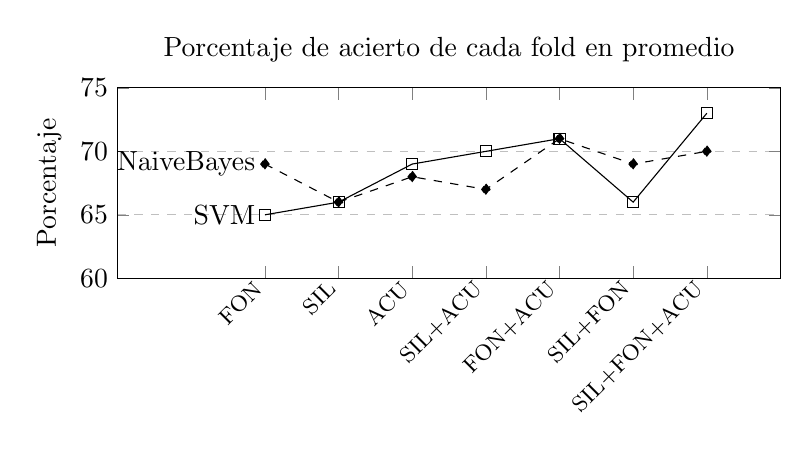
\begin{tikzpicture}

\begin{axis}[
    title={Porcentaje de acierto de cada fold en promedio},
    ylabel={Porcentaje},
    xmin=-1, xmax=8,
    ymin=60, ymax=75,
    xtick={1,2,3,4,5,6,7},
    xticklabels={FON,SIL,ACU,SIL+ACU,FON+ACU,SIL+FON, SIL+FON+ACU},
    x tick label style={rotate=45, anchor=east, font=\footnotesize},
    ytick={60,65,70,75},
    ymajorgrids=true,
    grid style=dashed,
] 

\addplot[mark=diamond*,dashed]coordinates {
    (1,69)(2,66)(3,68)(4,67)(5,71)(6,69)(7,70) };
\addplot[mark=square,solid,]coordinates {
    (1,65)(2,66)(3,69)(4,70)(5,71)(6,66)(7,73) };

\node [left] at (axis cs: 1, 69) {NaiveBayes};
\node [left] at (axis cs: 1, 65) {SVM};

\end{axis}
\end{tikzpicture}
\caption{Gráfico combinando distintos grupos de atributos}
\label{comb_atrib_graf}
\end{figure}

Lo esperable es que aumentando la cantidad de atributos se aumente el porcentaje de instancias  clasificadas correctamente. Esta idea se comprueba ya que la combinación que obtuvo mejor porcentaje fue $SIL+FON+ACU$ para el clasificador Support vector machine. En segundo lugar salió la combinación de $FON+ACU$ para ambos clasificadores y en tercero $SIL+ACU$ sólo para Support vector machine. 

Podemos notar que el tipo de atributo que posee mayor presencia es el que corresponde a los atributos acústicos ($ACU$), ya que se encuentran en los tres primeros grupos de atributos que obtuvieron mejor porcentaje (estos son: $SIL+FON+ACU$, $FON+ACU$ y $SIL+ACU$). Quizás entre los atributos acústicos no haya uno con información predominante, pero la combinación de todos los atributos de esa clase hace que los clasificadores tengan buenas métricas.